\documentclass[12pt,a4paper]{article}
\usepackage[utf8]{inputenc}
\usepackage[spanish]{babel}
\usepackage{amsmath}
\usepackage{amsfonts}
\usepackage{amssymb}
\usepackage{makeidx}
\usepackage{graphicx}
\usepackage{lmodern}
\usepackage{kpfonts}
\usepackage{apacite}
\usepackage{multirow}
\usepackage{graphicx}
\usepackage[svgnames]{xcolor}
\usepackage{listings}

\lstset{language=R,
    basicstyle=\small\ttfamily,
    stringstyle=\color{DarkGreen},
    otherkeywords={0,1,2,3,4,5,6,7,8,9},
    morekeywords={TRUE,FALSE},
    deletekeywords={data,frame,length,as,character},
    keywordstyle=\color{blue},
    commentstyle=\color{DarkGreen},
}
\setlength{\parindent}{0em}
\usepackage[left=3cm,right=3cm,top=2cm,bottom=2cm]{geometry}
\author{Pablo Vivas Corrales\footnote{\textit{Maestría Académica en Estadística. Universidad de Costa Rica}}\\\textit{pablo.vivas@ucr.ac.cr}}
\title{Distribución Gompertz-Weibull Flexible}
\date{23 de noviembre de 2020}
\begin{document}
\maketitle
\begin{abstract}
\noindent
La distribución Gompertz-Weibull Flexible (GoFW) surge como una alternativa para abordar, principalmente, análisis de supervivencia cuando la tasa de ocurrencia del evento no es monótona. Con el objetivo de descubrir características de esta distribución, que es relativamente nueva, bajo cierto escenarios y cuantificar su desempeño con análisis empírico, se realiza una serie de simulaciones y se analizan un conjunto de datos reales. Las estimaciones de los parámetros se realizan mediante máxima verosimilitud y métodos numéricos como el algoritmo de Newton-Raphson. Por medio de simulaciones, se analiza la potencia de los coeficientes $\beta_0$ y $\beta_1$. Esto se realiza variando el tamaño de muestra (n) de 1 a 500 elementos y calculando la potencia mediante 100 iteraciones por tamaño de muestra. También se analiza  el rendimiento de este modelo contra modelos paramétricos (Weibull y Exponencial) con datos simulados y datos reales. Se varía el tamaño de muestra de 10 a 500 y además se utiliza el criterio de AIC para selección de modelos. Se encuentra lo siguiente: la potencia de este modelo es bastante alta para cualquier tipo de tamaño de muestra, para un tamaño de muestra más alto de 100, la potencia es práctiamente 1, el modelo GoFW se debe seleccionar ante los modelos Weibull y Exponencial, si se sopecha que los datos provienen de una mezcla de distribuciones. \\
\\
\textbf{Palabras clave:} \textit{Distribución Gompertz-Weibull Flexible, Simulaciones Análisis Empírico \& Máxima Verosimilitud} 
\end{abstract}

\section{Introducción}

La familia de distribuciones Weibull son ampliamente conocidas y utilizadas en estadística, ingeniería y otros campos del conocimiento, para describir el comportamiento de fenómenos aleatorios, específicamente,  para analizar tiempos o duraciones a un evento (análisis de sobreviviencia) o modelizar el riesgo de eventos o situaciones extremas o atípicas (análisis de valores extremos). Desde su amplia caracterización en 1951 por  Waloddi Weibull, casos específicos de esta distribución, como la distribución exponencial y la distribución Rayleigh, se han utilizado para abordar preguntas científicas.\\
\\
Esta familia de distribuciones son adecuadas en análisis de sobreviviencia con tasas de fallas (ocurrencia del evento) monótonas (Ahmad e Iqbal, 2017), es decir, con fallos que se presentan con un patrón creciente o decreciente. En su contraparte, su desempeño con fenómenos que no cumplen ese criterio es deficiente y por ese motivo se han desrrollado alternativas para atacar esta debilidad. Algunos ejemplos de estas alternativas son: distribución Weibull Flexible, distribución inversa Weibull-Gausiana y distribución Gompertz Weibull, entre otras.\\
\\
De las opciones antes mencionadas, se han dedicado una cantidad nada despreciable de artículos científicos a la distribución Weibull Flexible, esto por sus aplicaciones en análisis de confiabilidad, ensayos clínicos y experimentos de prueba de vida. Asimismo, con el objetivo de desarrollar una distribución aún más flexible y versátil, el estudio de esta distribución se ha combinado con la familia de distribuciones Gompertz, dando como origen la distribución Gompertz-Weibull Flexible, o GoFW por sus siglas en inglés.\\
\\
La distribución GoFW fue presentada en (Khaleel, M. A et al, 2020.), donde se establece desde su función de densidad hasta medidas de posición y variabilidad, incluso se realiza un estudio con datos reales y comparan su rendimiento con distribuciones similares. Sin embargo, al ser relativamente nueva, se necesita un mayor análisis de su comportamiento en diversos escenarios. Por esta razón, en este documento se realiza un análisis de la distribución GoFW, bajo el enfoque de simulaciones y además se elabora un análisis con datos reales, todo lo anterior con los siguiente objetivos: descubrir características de esta distribución bajo cierto escenarios y cuantificar su desempeño con datos reales.\\
\\
Para cumplir dichos objetivos, este trabajo se estructura de la siguiente forma: en la sección de métodos se profundiza sobre la especificación del modelo a estudiar y su función de verosimilitud para la estimación de los parámetros, luego se especifícan los escenarios sobre los cuales se realizan las simulaciones y se menciona los datos utilizados para el ejemplo empírico. En la sección de resultados se presentan las características encontradas en los análisis y en la sección de conclusiones se destacan los resultados más llamativos derivados de los análisis.


\section{Métodos}
La función de distribución y la función de densidad de una variable aleatoria \textit{t}, que sigue una distribución Gompertz-Weibull Flexible están dadas por las siguientes ecuaciones:
\begin{equation}
F(t)= 1-e^{\left( \frac{\theta}{\gamma}\right )\left \{1- \left [ exp \left ( -e^{\alpha t - \frac{\eta}{t} } \right ) \right ]^{-\gamma} \right \}}
\end{equation}

\begin{equation}
f(t)= \theta \left ( \alpha + \frac{\eta}{t^2} \right ) e^{\alpha t - \frac{\eta}{t}} \left [ exp \left ( -e^{\alpha t - \frac{\eta}{t} } \right ) \right ]^{-\gamma} e^{\left( \frac{\theta}{\gamma}\right )\left \{1- \left [ exp \left ( -e^{\alpha t - \frac{\eta}{t} } \right ) \right ]^{-\gamma} \right \}}
\end{equation}

para $\alpha, \eta, \theta$ y $\gamma > 0$. Sin embargo, se realiza la siguiente modificación $\eta = exp(\beta_0+\beta_1\cdot X)$ para darle un enfoque de modelos lineales.\\
\\
Asismismo, las funciones de sobreviviencia y de hazard están dadas por las siguientes expresiones:
\begin{equation}
S(t)= e^{\left( \frac{\theta}{\gamma}\right )\left \{1- \left [ exp \left ( -e^{\alpha t - \frac{\eta}{t} } \right ) \right ]^{-\gamma} \right \}}
\end{equation}
\begin{equation}
h(t)= \theta \left ( \alpha + \frac{\eta}{t^2} \right )e^{\alpha t - \frac{\eta}{t} }\left [ exp \left ( -e^{\alpha t - \frac{\eta}{t} } \right ) \right ]^{-\gamma}
\end{equation}

Para realizar la estimación de los parámetros se utiliza el procedimiento de máxima verosimilitud, por lo que se necesita definir esta función para una muestra específica. Además, se trabaja con el logaritmo natural de esta función para simplificar ciertos cálculos.  A partir de la función de densidad se puede derivar la siguiente función de log-verosimilitud:
\begin{gather}
l(\alpha, \eta, \theta, \gamma;t_{i}) = n \log(\theta)+ \sum_{i=1}^{n} \log \left ( \alpha+\frac{\eta}{t_{i}^{2}}\right )+  \sum_{i=1}^{n}\left ( \alpha t_{i}-\frac{\eta}{t_{i}}\right ) + \nonumber\\ \gamma \sum_{i=1}^{n} exp\left ( \alpha t_{i}-\frac{\eta}{t_{i}}\right) 
 + \left( \frac{\theta}{\gamma}\right ) \left \{1- \left [ exp \left ( -e^{\alpha t_i - \frac{\eta}{t_i} } \right ) \right ]^{-\gamma} \right \} 
\end{gather}

La estimación por máxima verosimilitud de los parámetros $\alpha, \eta, \theta$ y $\gamma$ se obtienen resolviendo similtáneamente las siguientes ecuaciones: $\frac{\partial l}{\partial \alpha} =0$, $\frac{\partial l}{\partial \eta} =0$, $\frac{\partial l}{\partial \theta} =0$ y $\frac{\partial l}{\partial \gamma} =0$. Sin embargo, estas soluciones no pueden obtenerse de forma analítica y se necesita emplear métodos numérticos como el algoritmo de Newton-Raphson.\\
\\
Por medio de simulaciones, se analiza la potencia de los coeficientes $\beta_0$ y $\beta_1$. Esto se realiza variando el tamaño de muestra (n) de 1 a 500 elementos y calculando la potencia mediante 100 iteraciones por tamaño de muestra. Cabe resaltar que se emplea la técnica de muestreo de transformación inversa para generar muestras de esta distribución de probabilidad. También se analiza  el rendimiento de este modelo contra modelos paramétricos (Weibull y Exponencial) con datos simulados y datos reales. Se varía el tamaño de muestra de 10 a 500 y además se utiliza el criterio de AIC para selección de modelos. Es menester destacar que en la creación de datos se simulan los siguientes escenarios: datos con distribución GoFW, datos con distribución Weibull, datos con distribución exponencial y datos con distribución de mezcla de dos distribuciones Weibull.\\
\\
Para la realización  de las simulaciones y el proccesamiento de los datos se utilizó el software R en su versión 4.0.2 y el IDE RStudio en su versión 1.3.1075. Los paquetes de R utilizados fueron los siguientes: readxls, dplyr, ggplot2, stats4 y survival. Toda la información de este documento(datos, análisis y resultados) se encuentra disponible en un repositorio de Github que se puede accesar mediante esta dirección: https://github.com/pablo-vivas/Proyecto-MLG.
\newpage
\section{Resultados}
En esta sección se muestra, para cada uno de los escenarios descritos con anterioridad los resultados de
la simulaciones con respecto a la potencia de los coeficientes $\beta_0$ y $\beta_1$ y la preferencia mediante el criterio del AIC para cada uno de los tres modelos estimados. 

\begin{figure}[h!]
\begin{center}
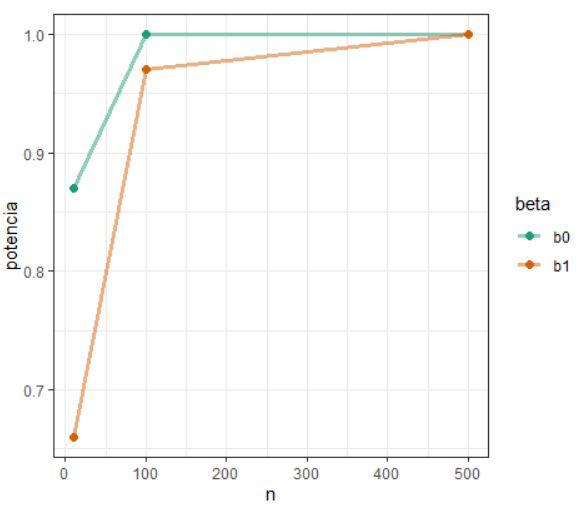
\includegraphics[scale=0.75]{potencia.JPG} 
\caption{Potencia de los coeficientes $\beta_0$ y $\beta_1$ de una distribución Gompertz-Weibull Flexible}
\end{center}
\end{figure}

Como se puede observar de la Figura 1, tanto el intercepto ($\beta_0$) como el coeficiente de $\beta_1$ tienen una potencia bastante alta para todos los tamaños de muestra. Es decir, que para la mayoría de las iteraciones (100 iteraciones), se concluyó que el intercepto y el otro coeficiente eran significativamente distintos de cero. Se aprecia que la potencia de los coeficientes aumenta con el tamaño de la muestra, aunque para tamaños de muestras pequeños, la potencia del coeficiente $\beta_1$ sigue siendo relativamente alta. Asimismo, se debe mencionar que este es un caso especial dela distribución GoFW, cuando los parámetros son igual a 1 y los coeficientes $\beta_0$ y $\beta_1$ son 2 y 0,5, respectivamente. Se decidió utilizar esta configuración por problemas en la convergencia del modelo y problemas en la generación de observaciones aleatorias que sigan esta distribución. También cabe mencionar que para la variable independiente se generaraon observaciones que provenían de una distribución Bernoulli con una probabilidad de éxito de 0,5.
\newpage

\begin{figure}[h!]
\begin{center}
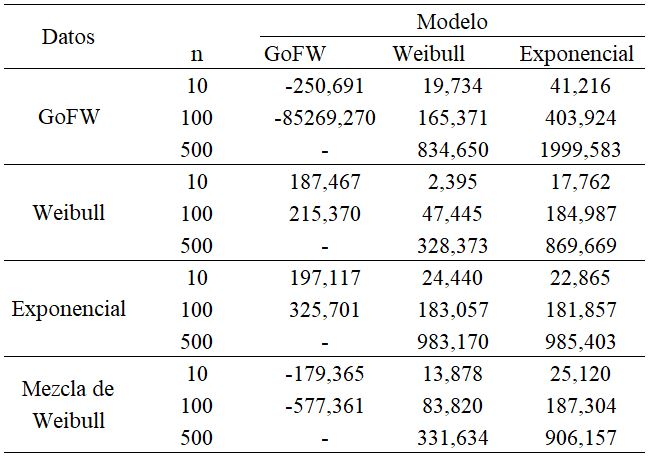
\includegraphics[scale=0.75]{tala1.JPG}  
\caption{Criterio AIC para selcción de modelos, en función de los datos generados, el tamaño de muestra y ell modelo empleado}
\end{center}
\end{figure}

En la figura dos se muestra el comportamiento del criterio del AIC para la selección de modelos. A partir de dicha figura se observa, como era de esperarse, que los modelos cuyos datos son generados para una distribución específica, tienden a ser mejores (bajo este criterio) que los otros, sin embargo, hay varios resultados interesantes: el modelo Weibull es mejor al modelo Exponencial cuando el tamaño de muestra es grande (n=500), además que el modelo GoFW se debe seleccionar ante los modelos Weibull y Exponencial, si se sopecha que los datos provienen de una mezcla de distribuciones Weibull. Esto último concuerda con lo establecido inicialmente sobre la utilidad de este modelo en eventos cuya función de riesgo no sea monótona.\\
\\
Otro aspecto clave que se deriva de esa figura, es que el modelo GoFW tiene problemas de convergencia cuando el tamaño de muestra es grande. En la generación de datos que siguen esta distribución se utilizaron otros parámetros de $\alpha, \theta$ y $\gamma$, distintos a usados en la figura 1, esta es la razón por la cual se tuvo problemas en la convergencia de este modelo, por lo tanto se afirma que el modelo GoFW es sensible a los cambios en sus parámetros.\\
\\
Para el análisis empírico se utiliza información sobre el tiempo de falla de 84 parabrisas de avión. Estos datos fueron recopilados originalmente por (Tahir, M. H. et al, 2015) y fueron modificados por (Zubair Ahmad, 2017), asimismo se decide incluir para efectos de este trabajo, una nueva variable que representará el tipo de avión, esto se hace para poder hacer el ajuste del modelo GoFW tal y como se ha trabajado durante todo el documento. 
\newpage

\begin{figure}[h!]
\begin{center}
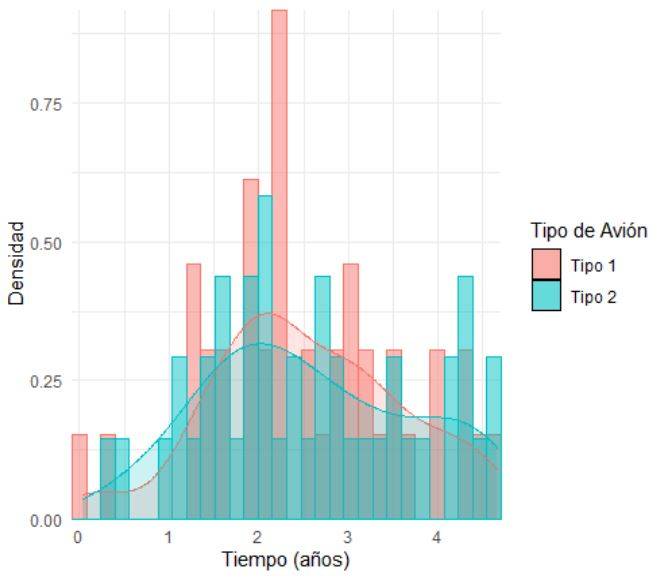
\includegraphics[scale=0.68]{avion.JPG} 
\caption{Potencia de los coeficientes $\beta_0$ y $\beta_1$ de una distribución Gompertz-Weibull Flexible}
\end{center}
\end{figure}

La estimación de los parámetros del modelo GoFW para este caso son los siguientes: $\hat{\alpha} = 0,7424 , \hat{\gamma}=0,3115, \hat{\theta}=1,0297, \hat{\beta_0}=0,3863$ y  $\hat{\beta_1}=0,7558$. Al realizar la comparación con el criterio del AIC, comparándo con los otros modelos antes establecidos, se tienen los siguientes resultados: -145,81; 265,99 y 239,74; para los modelos GoFW, Weibull y Exponencial, respectivamente, es decir, al igual que se observó en las simulaciones, esta distribución supera en rendimiento a las distribuciones Weibull y Exponencial. 


\section{Conclusiones}

La distribución Gompertz-Weibull Flexible (GoFW) es una de las tantas posibilidades para tratar de abordar fenómenos cuya tasa de ocurrencia del evento no es monótona. Esta función es relativamente nueva y es necesario estudiar sus propiedades estadísticas. En este trabajo se abordó una modificación del modelo original, esto para darle un enfoque de modelos lineales generalizados. A partir del análisis realizado, se concluye que la potencia de este modelo es bastante alta para cualquier tipo de tamaño de muestra, específicamente para un tamaño de muestra más alto de 100, la potencia es práctiamente 1. Por otro lado el modelo GoFW se debe seleccionar ante los modelos Weibull y Exponencial, si se sopecha que los datos provienen de una mezcla de distribuciones Weibull, asimismo este modelo tiene problemas de convergencia cuando el tamaño de muestra es grande. Una limitación importante de este estudio y el estudio original de donde proviene esta distribución, es la especificación de los parámetros para realizar simulaciones. En ambos documentos se establecen parámetros con un cierto patrón (que tengan el mismo valor) para que la generación de muestras aleatorias sea plausible, por lo tanto, se están dejando por fuera, un sinfín de escenarios para esta distribución.

\section{Anexos}

\subsection*{Referencias Biliográficas}
Ahmad, Z. and Hussain, Z. (2017). On transmuted Flexible Weibull extension distribution with applications to different lifetime data sets. American Journal of Computer Sciences and Applications, 1(1):1-12.\\
\\
Khaleel, M. A., Oguntunde, P. E., Ahmed, M. T., Ibrahim, N. A., and Loh, Y. F., (2020). Gompertz flexible Weibull distribution and it applications. Malaysian Journal of Mathematical Sciences, vol. 14, pp. 169-190.\\
\\
R Core Team. (2019). R: A language and environment for statistical computing [Manual de software inform´atico]. Vienna, Austria. Descargado de https://www.R-project.org/\\
\\
Tahir, M. H., Cordeiro, G. M., Mansoor, M. and Zubair, M (2015). The Weibull-Lomax Distribution: Properties and Applications', Hacettepe Journal of Mathematics and Statistics. \\
\\
Wickham, H. (2017). tidyverse: Easily install and load the ’tidyverse’ [Manual de software inform´atico]. Descargado de https://CRAN.R- 14 project.org/package= tidyverse (R package version 1.2.1) \\
\\
Wickham, H., y Bryan, J. (2019). readxl: Read excel files [Manual de software informático]. Descargado de https:/ CRAN.Rproject. org/package=readxl (R package version 1.3.1)\\
\\
Zubair Ahmad, Zawar Hussain. (2017) The New Extended Flexible Weibull Distribution and Its Applications. International Journal of Data Science and Analysis. Vol. 3, No. 3, 2017, pp. 18-23. doi: 10.11648/j.ijdsa.20170303.11

\subsection*{Código Utilizado}
\begin{verbatim}
# Trabajo Final  ----------------------------------------------------------

##Distribución Gompertz Flexible Weibull (GoFW)
##(Se ajusta $\eta$ para linealizarla)
## $\eta = exp(\beta_0+\beta_1*x)$

library(dplyr)
library(readxl)
library(ggplot2)
library(stats4)
library(survival)


# Log - Verosimilitud -----------------------------------------------------

ll_gofw <- function(alpha, beta0, beta1, gamma, theta){
  n = length(y)
  vero = suppressWarnings(n*log(theta) + sum(log(alpha+(exp(beta0 + beta1*x))
  /y^2)) +
    sum(log(alpha*y^2-(exp(beta0 + beta1*x))/y)) +
    gamma * sum(exp(alpha*y-(exp(beta0 + beta1*x))/y)) + 
    (theta/gamma) * (1-(exp(-exp(alpha*y-(exp(beta0 + beta1*x))/y)))^-gamma))
  log_vero = -sum(vero)
  return(log_vero)
}

# Potencia ----------------------------------------------------------------


#Caso particular Parámetros igual a 1

gen_gofw <- function(n, b_0 = 2, b_1 = 0.5){
  u = runif(n)
  x =  rbinom(n,1,0.5)
  p = -log(log(1-log(1-u)))
  t = (-p+sqrt(p**2+4*exp(b_0+b_1*x)))/2
  return(list(t=t,x=x))
}


pot_gofw <- function(it=100, n){
  pot_b0 = NULL
  pot_b1 = NULL
  for (i in 1:it){
    datos = gen_gofw(n)
    m = mle(ll_gofw, start = list(alpha = 1, beta0 =0 , 
                                  beta1=0, gamma=1, theta= 1))
  pot_b0[i] = 1*(prod(summary(m)@coef[2,1]+c(-2,2)*summary(m)@coef[2,2]) > 0)
  pot_b1[i] = 1*(prod(summary(m)@coef[3,1]+c(-2,2)*summary(m)@coef[3,2]) > 0)
  }
  p_b0=mean(pot_b0)
  p_b1=mean(pot_b1)
  return(list(p_b0=p_b0, p_b1=p_b1))
}

n <- seq(1,500,10)
p1 <- NULL
p2 <- NULL
for(j in n){
  p1[j] <- pot_gofw(n=j)$p_b0
  p2[j] <- pot_gofw(n=j)$p_b1
}

# Selcción de modelo

data <- data.frame(
  t = gen_gofw(10)$t,
  e = c(rep(1,10)),
  x = gen_gofw(10)$x
)
so <- Surv(time = data$t, event = data$e)
m_wei <- survreg(so ~ data$x, data = so, dist="weibull")
m_exp <- survreg(so ~ data$x, data = so, dist="exponential")
y <- data$t
x <- data$x
m_gofw <- mle(ll_gofw, start = list(alpha = 1, beta0 =0 , 
                                    beta1=0, gamma=1, theta= 1))
c(AIC(m_gofw),AIC(m_wei),AIC(m_exp))

datos_pot <- read_excel("datos_pot.xlsx",sheet = "Hoja2")

datos_pot$beta <- factor(datos_pot$beta)
str(datos_pot)

ggplot(datos_pot,aes(x=n,y=potencia,group=beta)) +
  geom_line(aes(colour=beta),size=1.2,alpha=0.5) +
  geom_point(aes(colour=beta),size=2.2) +
  scale_color_brewer(palette="Dark2")+
  theme_bw()

avion <- read_excel("avion.xlsx", sheet = "Hoja1")

ggplot(avion, aes(x = t, color = as.factor(x),
                  fill = as.factor(x) )) +
  geom_histogram(aes(y =..density..), alpha=0.5, 
                 position="identity") +
  geom_density(alpha=.2) +
  xlab("Tiempo (años)") + ylab("Densidad") +
  scale_fill_discrete(name = "Tipo de Avión", 
                      labels = c("Tipo 1", "Tipo 2")) + 
  guides(color = FALSE) +
  scale_y_continuous(expand = c(0,0)) +
  scale_x_continuous(expand = c(0,0)) +
  theme_minimal()
\end{verbatim}

\end{document}


